\documentclass[a4paper]{article}

\usepackage[T1]{fontenc}
\usepackage[italian]{babel}
\usepackage[latin1]{inputenc}
\usepackage{graphicx}
\usepackage{float}
\usepackage[margin=2 cm]{geometry}
\usepackage{multirow}
\usepackage{multicol}
\usepackage{color}
\author{Alberto Bordin, Giulio Cappelli}
\title{Analizzatore di spettro}
\date{27-28 novembre 2017}

\begin{document}
	\maketitle
	
\begin{abstract}
	Misura della separazione in frequenza dei modi di un laser HeNe.
	
	Misura della finezza di un Fabry-Perot.
\end{abstract}

\section{To do}

\begin{itemize}
	\item dire nella teoria che FSR e $\Delta\nu$ li riportiamo per semplicit� in unit� di tempo
\end{itemize}

\begin{multicols}{2}

\section{Teoria}

\subsection{Laser HeNe}

\subsection{Fabry-Perot}

\section{Apparato sperimentale}

\end{multicols}
	
\section{Modi del laser HeNe}

\begin{figure}[H]
	\centering
	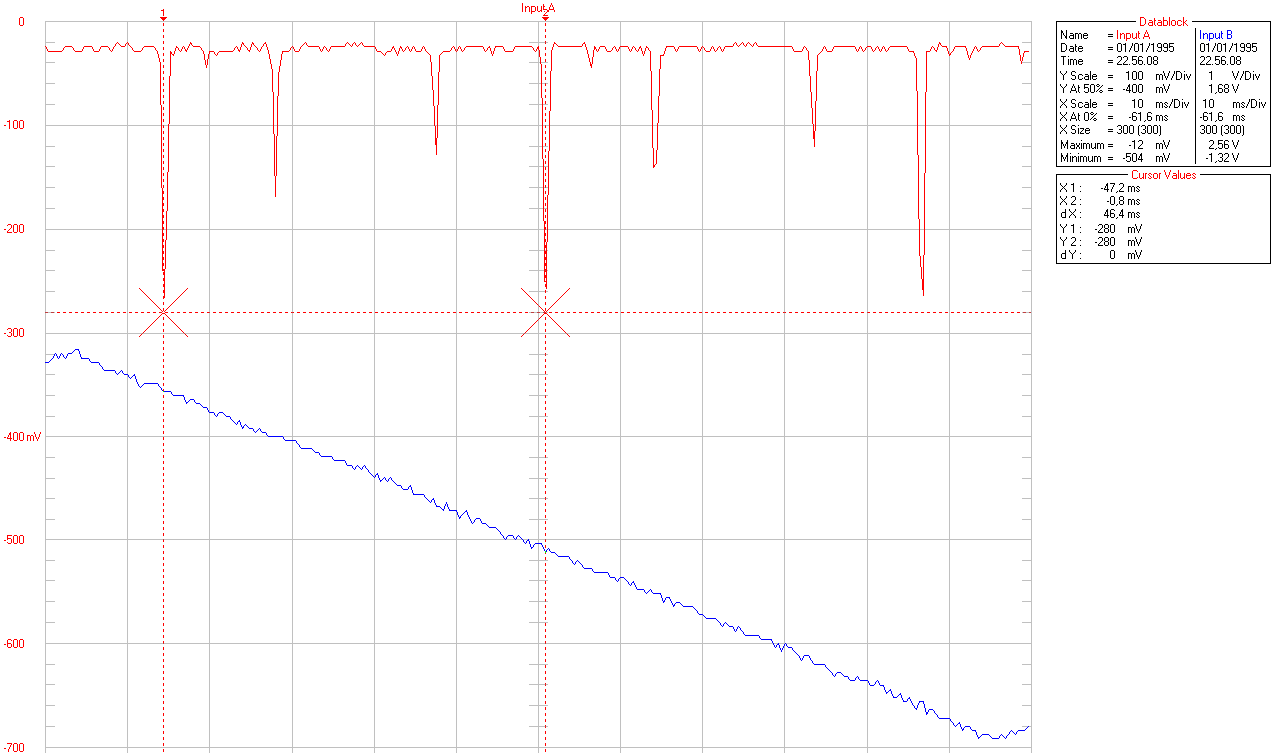
\includegraphics[width=1\textwidth]{due_ordini.png}
	\caption{Due ordini dell'analizzatore. In rosso i picchi di trasmittivit� della cavit� Fabry-Perot e in blu la rampa del generatore di funzioni.}
	\label{fig:due_ordini.png}
\end{figure}

\begin{figure}[H]
	\centering
	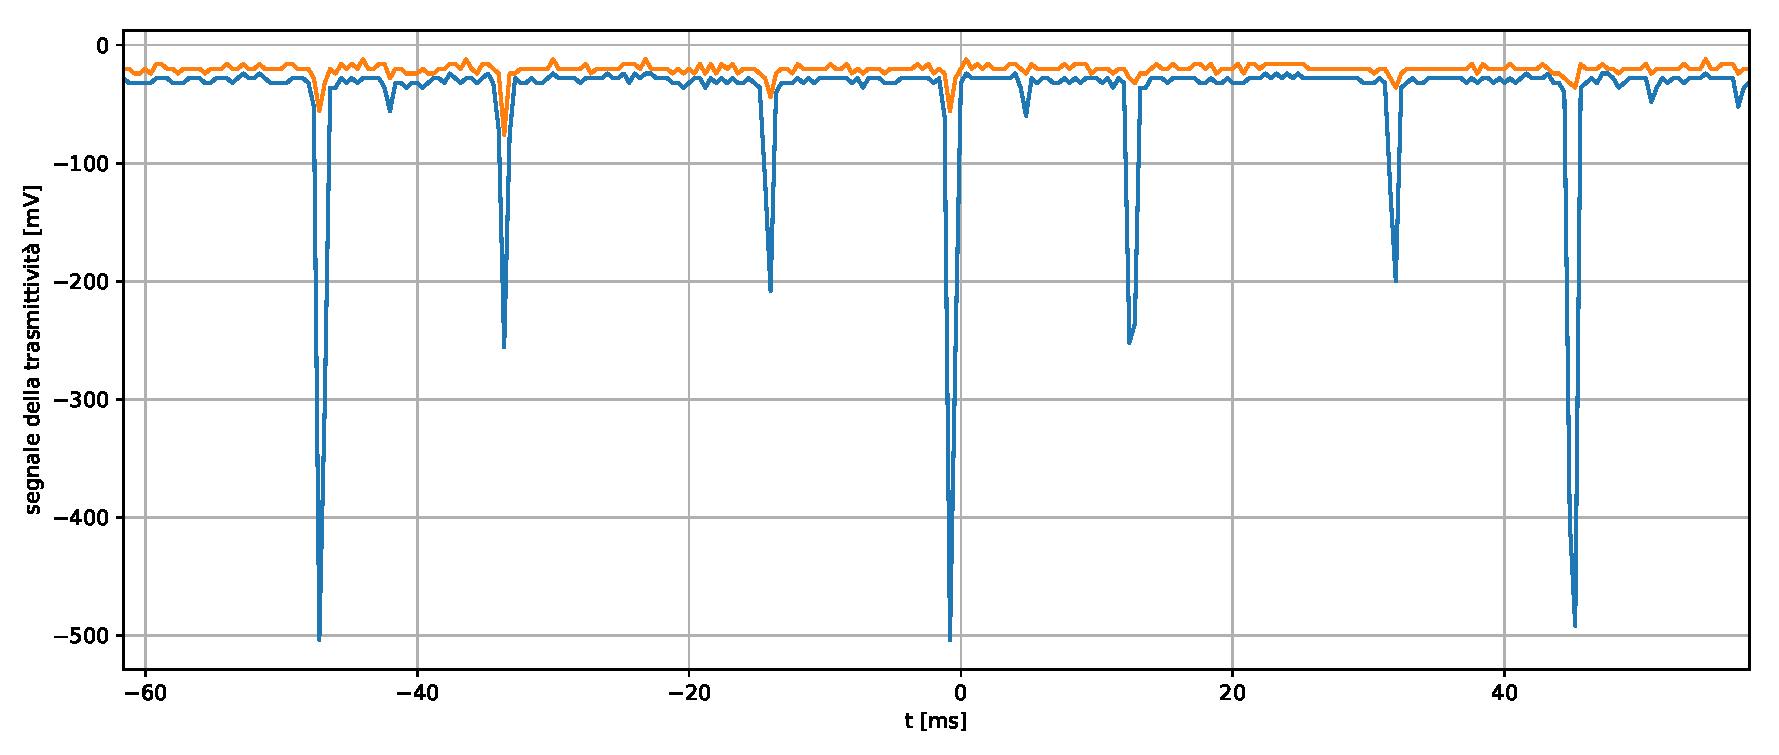
\includegraphics[width=1\textwidth]{due_ordini.pdf}
	\caption{Due ordini dell'analizzatore. Segnale di trasmittivit� salvato nel file .txt.}
	\label{fig:due_ordini.pdf}
\end{figure}

\begin{multicols}{2}
Analizziamo la separazione in frequenza dei modi del laser HeNe a nostra disposizione.

\subsection{Presa dati}

In Figura \ref{fig:due_ordini.png} vediamo un esempio del segnale letto dall'oscilloscopio e visualizzato al PC, e che salviamo anche in formato .txt. Sia per la trasmittivit� che per la rampa il file di testo riporta due diversi valori di tensione (vedi Figura \ref{fig:due_ordini.pdf}). Notiamo che il segnale visualizzato all'oscilloscopio � la media dei due. Inoltre, confrontando varie prese dati, notiamo che la discrepanza tra i due valori di tensione diminuisce notevolmente all'aumentare della larghezza del picco. Poich� per la misura della separazione in frequenza dei modi � importante la precisione sul tempo di ogni picco scegliamo di utilizzare il segnale pi� ampio al posto della media dei due.

In Figura \ref{fig:un_ordine.png} � riportato un'ordine dell'analizzatore.

\subsubsection{Accorgimenti sperimentali}
\begin{itemize}
	\item 
\end{itemize}

\end{multicols}

\begin{figure}[H]
		\def\svgwidth{1\textwidth}
		\input{un_ordine.pdf_tex}
		\caption{Un ordine dell'analizzatore.}
		\label{fig:un_ordine.png}
\end{figure}

\subsection{Analisi dati}

\begin{multicols}{2}
	
La FSR pu� essere stimata banalmente facendo la differenza tra i tempi di due picchi principali consecutivi. Avendo pi� di un ordine si pu� migliorare questa stima ad esempio facendo la media delle varie differenze tra picchi consecutivi oppure prendendo la differenza di tempo tra il primo e l'ultimo e divindendola per il numero di ordini, ma una stima ancora pi� precisa si pu� ottenere con un fit. Di seguito (e in Figura \ref{fig:esempio_deltanu}) riportiamo il procedimeto seguito:
\begin{itemize}
	\item tramite uno script in python estraiamo i tempi di ogni picco,
	\item facciamo un grafico "numero di ordine" - "tempo del picco",
	\item eseguiamo un fit lineare.
\end{itemize}
Come si deduce dalla presenza di tre rette parallele in Figura \ref{fig:esempio_deltanu} lo stesso procedimento � seguito per ognuno dei 3 modi visibili. Il coefficiente angolare della retta fittata � la FSR, mentre la differenza tra le intercette � il tempo corrispondente al $\Delta\nu$.
Quindi ricaviamo $\Delta\nu$ con la formula 
\[ \Delta\nu \textrm{ [Hz]}= 1500 \frac{\Delta\nu\textrm{ [ms]}}{FSR\textrm{ [ms]}}\]
Per ridurre ulteriormente l'errore, nel caso in cui le rette non fossero esattamente parallele, per la FSR prendiamo la media dei 3 coefficienti angolari misurati e la differenza tra le intercette la prendiamo a met� delle rette.

Fit e calcoli sono stati eseguiti con python 3, per brevit� riportiamo solo il valore di $\Delta\nu$ e lasciamo a disposizione il codice dello script al link in nota\footnote{https://github.com/albord95/relazioni-lab-ottica-quantistica/tree/master/Analizzatore\%20di\%20spettro/dati\%20e\%20script \\ Scaricare tutta la cartella ed eseguire il file modi\_laser\_HeNe.py. \'E necessario python 3 con i pacchetti pylab, scipy e gvar.}
	
\begin{figure}[H]
	\centering
	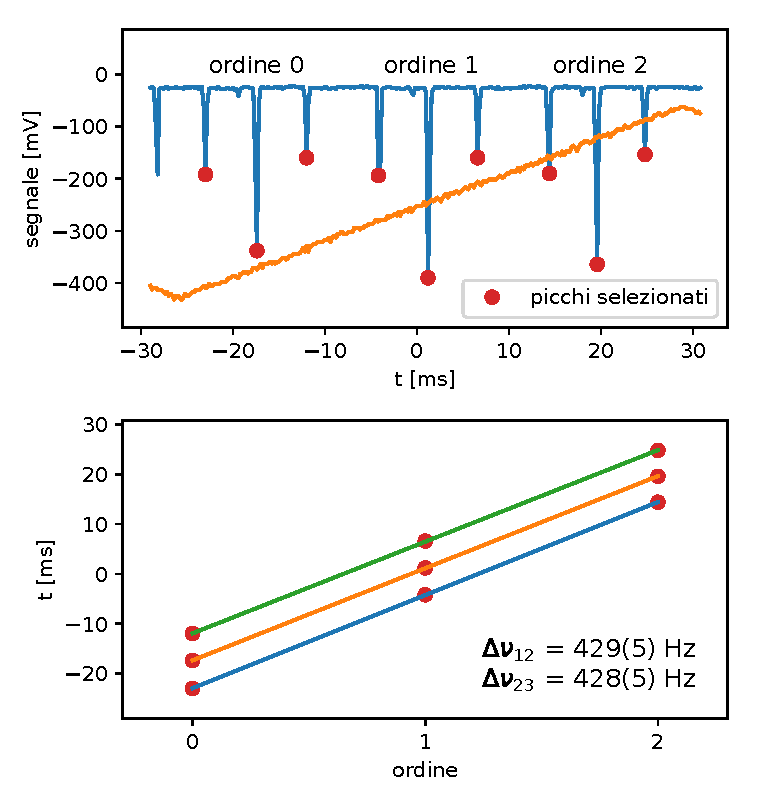
\includegraphics[width=0.5\textwidth]{esempio_deltanu.pdf}
	\caption{Esempio di analisi. In appendice sono riportate anche le restanti prese dati. La rampa del plot in alto � riscalata per questioni estetiche.}
	\label{fig:esempio_deltanu}
\end{figure}
	
\end{multicols}
	
\section{Finezza del Fabry-Perot}

\begin{multicols}{2}

\end{multicols}

\newpage
\centering
\section*{Appendice}

\begin{figure}[H]
	\makebox[\textwidth]{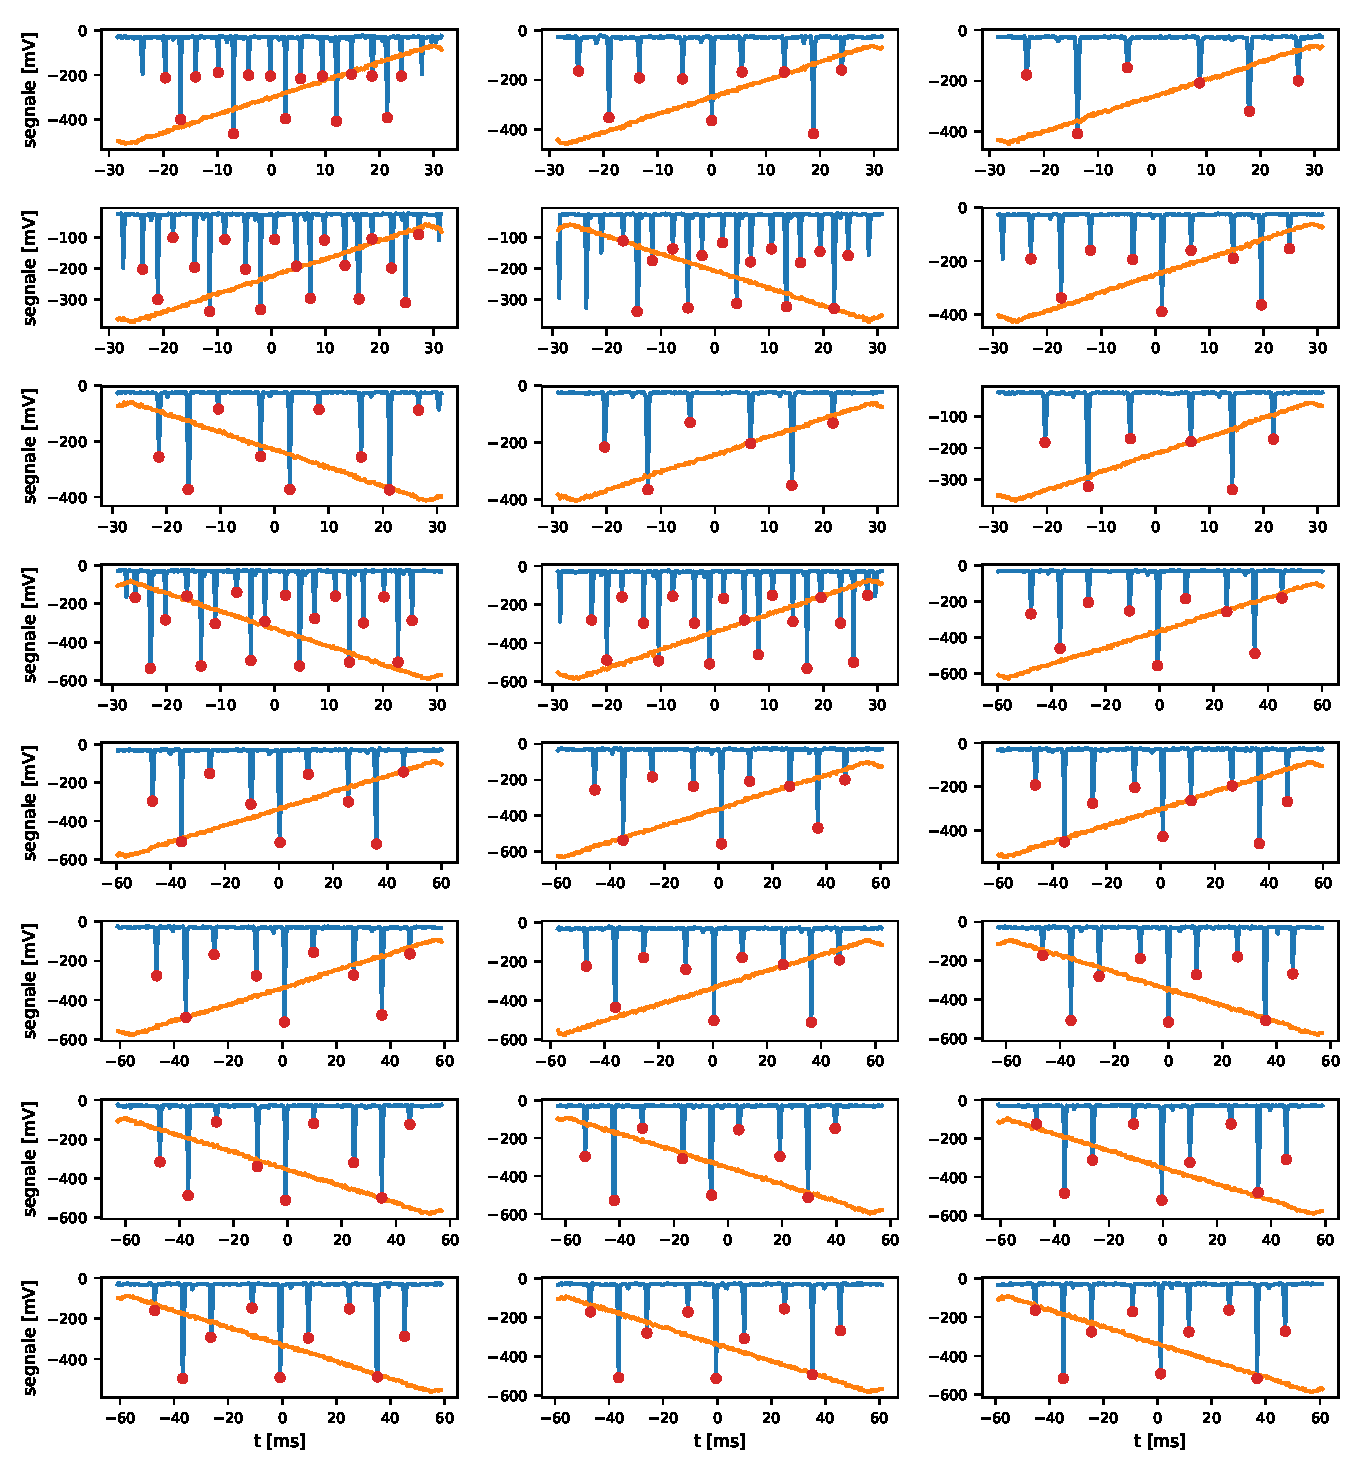
\includegraphics[width=1.18\linewidth]{24picchi.pdf}}
	\caption{Selezione dei tempi per i fit di Figura \ref{fig:24fit}.}
	\label{fig:24picchi}
\end{figure}

\begin{figure}[H]
	\makebox[\textwidth]{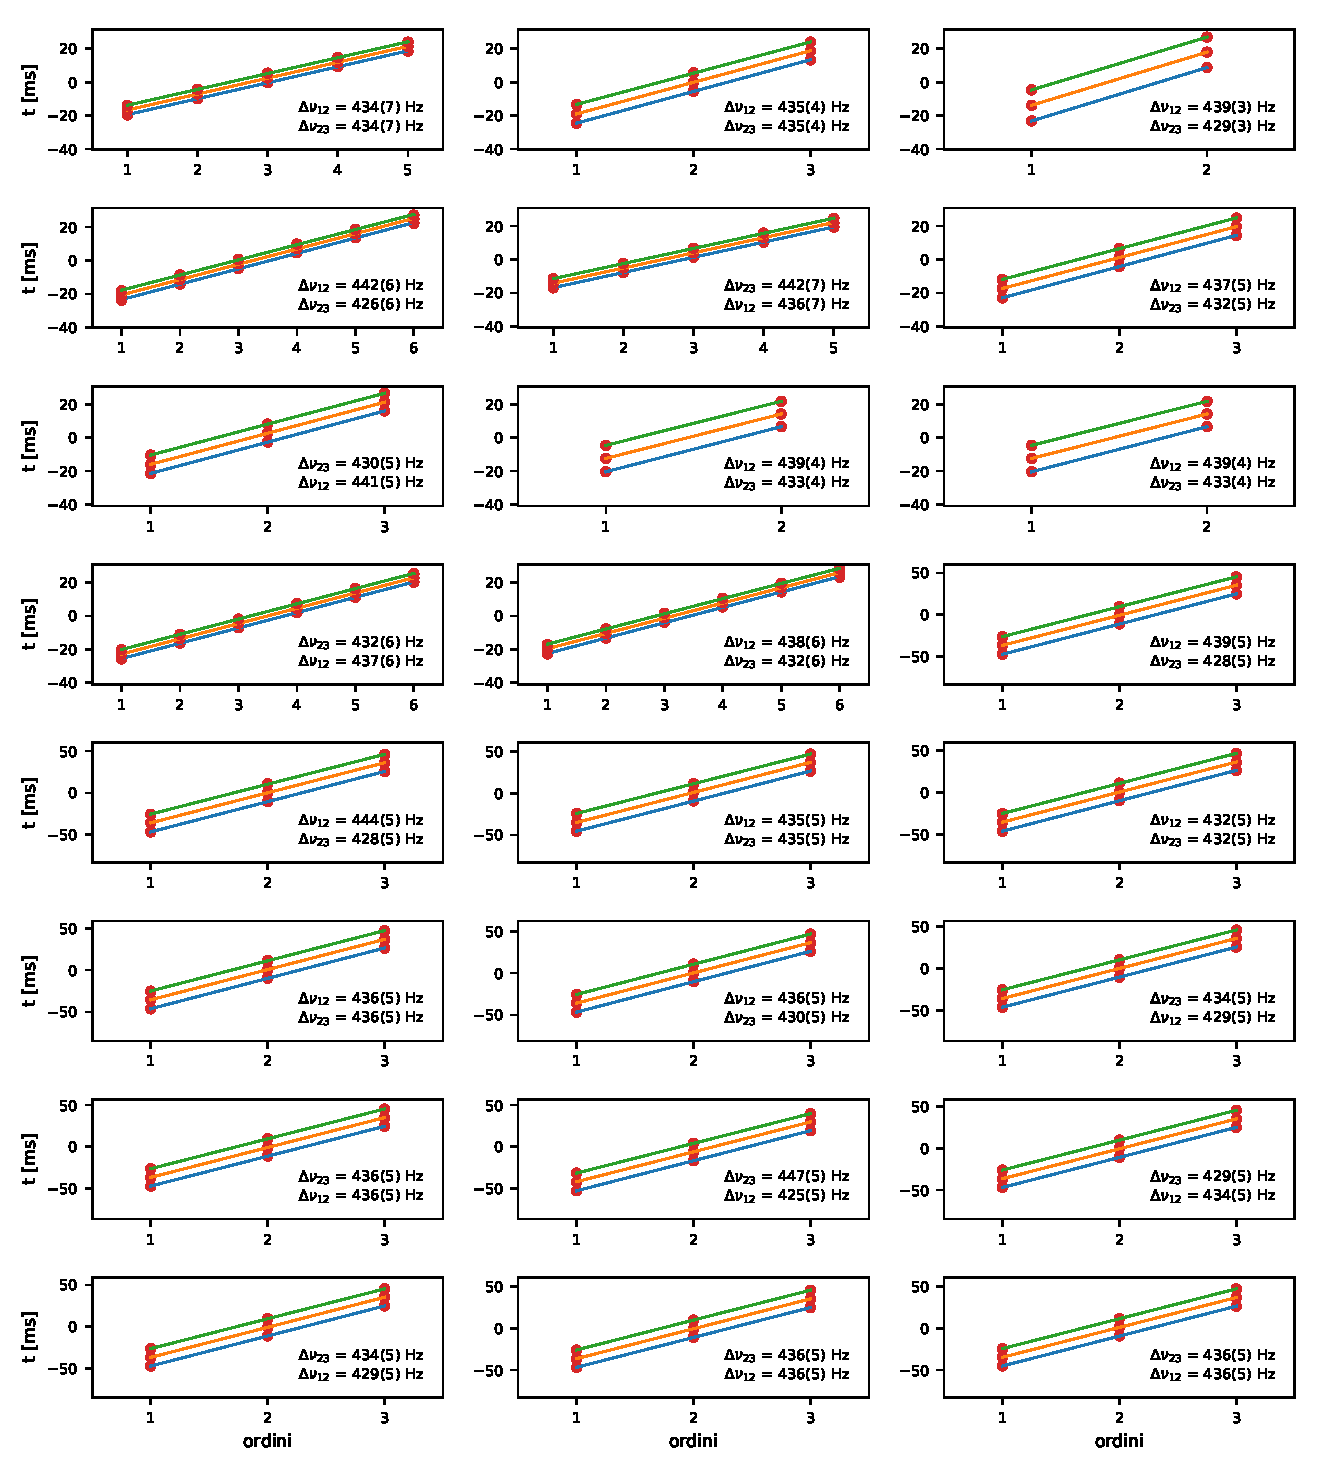
\includegraphics[width=1.18\linewidth]{24fit.pdf}}
	\caption{Fit e calcolo dei $\Delta\nu$.}
	\label{fig:24fit}
\end{figure}

	
\end{document}

